\title{Object Detection - Independent Study HTW Berlin}
\author{Jakob Pfeiffer}
\date{10.10.2018}
\begin{abstract}
Object Detection ist ein schnell wachsender Bereich innerhalb Computer Vision. Das Ziel von Object Detection ist es Objekte in Bilder sowohl zu klassifizieren als auch zu lokalisieren. State-of-the-Art Ansätze verwenden gewöhnlicherweise Convolutional Neural Networks mit verschiedenen Architekturen. Innerhalb dieser Individual Study wird versucht moderne Ansätze zur Object Detection im Detail zu verstehen und zu vergleichen. Speziell die Region Based Detectors. Weiterhin werden verschiedene Netzwerke ausprobiert und die Ergebnisse präsentiert.
\end{abstract}

\begin{document}
\tableofcontents 
\newpage
\section{Einleitung}\label{sec:einleitung}
 Für immer mehr Themen innerhalb der Computer Vision gibt es Ansätze mit neuronalen Netzen, meistens mit \textbf{Convolutional Neural Networks (CNN)}. Dazu gehören Klassifizierung, Face Recognition, Segmentierung und Object Detection. Das Ergebnis eines CNNs sind im Grunde Feature Tensoren eines Bildes, welche Formen, Farben etc. beschreiben.  Ein Convolutional Layer lässt lokale, rezeptive Felder (die Gewichte, oft 3-x-3) über ein Bild laufen und erstellt somit pro Gewicht eine zweidimensionale Feature Map. Die Tiefe der Feature Map wird über die Anzahl der Gewichte bestimmt. Normalerweise hat ein CNN mehrere von diesen Layern, was zu einer Hierarchie führt: die Features der ersten Layer sind sogenannte Low-Level Features und beschreiben Linien, Farben etc. Je mehr Layer benutzt werden, desto komplexer werden die Features (Kreise, Vierecke, Zylinder etc.) die entdeckt werden (High-Level Features), da es Kombinationen aus den Features der Layer davor sind. Die höchsten Layer finden dann einzelne Klassen von Objekten.  Diese grundlegende Architektur wird eben nicht nur bei der Klassifizierung (hier wird die Architektur noch um fully-connected Layer erweitert), sondern auch bei Object Detection und Segmentierung verwendet. Der Unterschied findet sich oft nur inder Art und Weise wie die Netzwerke trainiert werden und wie die Feature Tensoren verarbeitet werden.  \textbf{Object Detection} ergänzt die Klassifizierung von Objekten eines Bildes um die Lokalisierung innerhalb des Bildes. Meistens gegekennzeichent mit Bounding Boxen. Unterschieden wird vorallem zwischen \textit{Region Based Detectors} und \textit{Single Shot Detectors}. Region Based Detectors finden interessante Regionen eines Bildes, klassifizieren diese und verfeinern die Koordinaten, während Single Shot Detectors das Bild als Ganzes betrachten, das Bild unterteilen und versuchen, ausgehend von diesen gleichgroßen Teilen, Objekte zu klassifizieren \& zu lokalisieren. Innerhalb dieser Individual Study werden Region Based Detectors betrachtet.
\section{Region Based Detectors}\label{sec:regionBasedDetectors}
 Die bekannteste Architektur-Familie der Region Based Detectors ist \textbf{Regions with CNN Features} oder auch \textbf{R-CNN} \cite{girshick14CVPR}. Dazu gehören bzw. daraus entstanden ebenfalls \textit{Fast R-CNN}, \textit{Faster R-CNN} und \textit{Mask R-CNN}.  Alle diese Architekturen haben das gleiche Gerüst: die Eingabe ist ein Bild, welches zwei Prozessen unterzogen wird. Zum Einen werden relevante Features in dem Bild gefunden und entsprechend dargestellt, zum Anderen werden Regionen-Vorschläge (\textit{region proposals}) bestimmt. Im nächsten Prozess werden die Regionen-Vorschläge durch die gefundenen Features beschrieben. Nach einem weiteren Prozess, der diese Features verarbeitet, können eine beliebige Anzahl Networks-Heads angehangen werden. Jeder dieser Heads erfüllt dann eine bestimmte Funktion, oft können die Heads parallel ausgeführt werden.  Die Prozesse lassen sich aufteilen in Prozesse die pro Bild (relevante Features extrahieren, Regionen-Vorschläge erstellen) und in Prozess die pro Region (Regionen durch Features beschreiben, Regionen-Features verarbeiten, Networks-Heads) durchgeführt werden.\cite{generalizedrcnn} Die Unterschiede zwischen den Architekturen sind die Methoden, welche benutzt werden, um die einzelnen Prozesse durchzuführen. Eine Übersicht ist in Tabelle \ref{tbl:rcnnarchtable} gegeben.

\subsection{R-CNN/Fast R-CNN}
 Die erste Architektur, einfach \textbf{R-CNN} (mittlerweile auch: Slow R-CNN), hat aufwendige Methoden für die Prozesse pro Region (Forward-Pass durch CNN, c1-vs-rest-SVM, Box regression) und ist sehr langsam, da pro Bild ca. 2000 Regionen vorgeschlagen werden. Zusätzlich verlangt die Architektur während des Trainings die Feature-Vektoren pro Regionen zwischenzuspeichern und seperat, zu dem CNN, pro Klasse eine Support Vector Machine zu trainieren.\cite{girshick14CVPR}
\begin{table}[t]
\begin{tabular}{|l|c|c|c|c|}
\hline
Prozess/Architektur & \textbf{R-CNN} & \textbf{Fast R-CNN} & \textbf{Faster R-CNN} & \textbf{Mask R-CNN} \\ \hline
\textit{Feature Extraktion} & Identity & \textcolor{ForestGreen}{CNN} & CNN & CNN \\ \hline
\textit{Region Vorschläge} & Sel. Search & Sel. Search & \textcolor{ForestGreen}{RPN} & RPN\\ \hline
\textit{Regionen als Features} & Crop/Wrap & \textcolor{ForestGreen}{RoIPool} & RoIPool & \textcolor{ForestGreen}{RoIAlign}\\ \hline
\textit{Feature Verarbeitung} & CNN & \textcolor{ForestGreen}{MLP} & MLP & MLP\\ \hline

Network Heads & SVM & \textcolor{ForestGreen}{Softmax-Class.} & Softmax-Class. & Softmax-Class.\\
Network Heads & Box Regressor & Box Regressor & Box Regressor & Box Regressor\\
Network Heads & & & & \textcolor{ForestGreen}{Mask-Branch} \\ \hline

\end{tabular}
\caption{Verschiedene Region-Based Architekturen (\textcolor{ForestGreen}{Veränderungen}) \cite{generalizedrcnn}}
\label{tbl:rcnnarchtable}
\end{table}
\subsection{Faster R-CNN}\label{subsec:fasterR-cnn}
 Insgesamt gibt es somit \texttt{Anzahl Anchors x Anzahl Positionen} Regionen-Vorschläge. In der Regel sind das mehrere Tausend.
Während des Trainings wird eine Stichprobe von 256 Anchors erstellt, die einen Einfluss auf Loss und die Backpropagation hat. Im Idealfall enthält diese 128 positive Anchors\footnote{IoU mit Ground-Truth-Box \texttt{> 0.7}} und 128 negative Anchors\footnote{IoU \texttt{> 0.3} mit allen Ground-Truth-Boxen}. Oft gibt es weniger positive Anchors, dann wird die Sitchprobe mit negative Anchors aufgefüllt.
Durch die beschriebene Architektur ist es möglich akkurate Regionen-Vorschläge zu generieren, die unabhängig von der Größe von Objekten (\textit{scale-invariant}) und der Position von Objekte im Bild (\textit{translation-invariant}) interessante Gebiete im Bild finden. Somit wird eine solide Grundlage zur Object Detection geschaffen. In Tabelle \ref{tbl:resultsarch}
Durch die Integration eines Feature Pyramid Networks (FPN) können die Ergebnisse weiter verbessert werden. Dies wird in Kapitel \ref{subsec:fpn} weiter erläutert.
\subsection{Mask R-CNN}\label{subsec:maskrcnn}
 Im Grunde gibt es bei der Architektur des Mask R-CNN zwei wesentliche Veränderungen (im Vergleich zur Faster R-CNN Architektur):
\begin{itemize}
    \item der RoIPool-Layer wird mit dem \textit{RoIAlign-Layer} ersetzt
    \item es gibt einen zusätzlichen Head-Branch für die Segmentierung (\textit{Mask-Branch})
\end{itemize}
Der \textit{RoIAlign-Layer} ist wichtig für die pixel-genaue Segmentierung. Bei RoI-Pooling findet eine Quantisierung statt, die mit einem Genauigkeitsverlust einher geht. Dieser Verlust hat keinen großen Einfluss auf die Ergebnisse der Object Detection. Allerdings bei einer Segmentierung nach Pixel spielt die Genauigkeit eine weit größere Rolle und wird durch eine bilineare Interpolation der Feature Map - Werte erhöht im RoIAlign-Layer erhöht.
Der \textit{Mask-Branch} besteht aus einem Fully Convolutional Network. Diese Network enthält eine oder mehrere \textbf{De-Convolution Layer}, die die Feature-Map in Höhe und Breite vergrößern. Die Tiefe der letzten Feature-Map (für jede Region of Interest) entspricht der Anzahl der Klassen, somit gibt es für jede Klasse eine Art binäre Maske, die darstellt wo auf dem Bild (pixel-weise) ein Objekt ist.
Die restliche Architektur entspricht, mit kleinere Anpassungen (vor allem im Training), dem Faster R-CNN.
\begin{figure}[h]
%\centering
  %\centering
  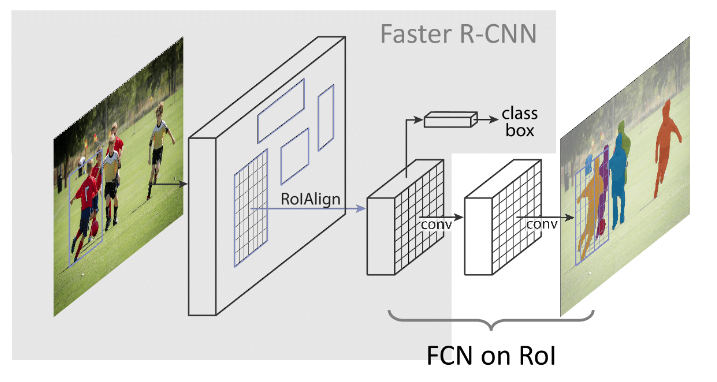
\includegraphics[width=.4\linewidth]{imgs/mask_rcnn.png}
  \caption{Mask R-CNN\cite{maskrcnnPresentation}}
\end{figure}
\label{img:mask_rcnn}
\begin{figure}[h]
  %\centering
  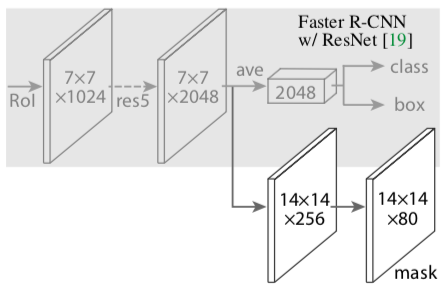
\includegraphics[width=.4\linewidth]{imgs/mask_branch.png}
  \caption{Mask Branch\cite{maskrcnn}}
\end{figure}
\label{img:mask_branch}

\newpage

\end{document}